To validated that the cluster gives us an improvement when working on big data, a list of tests will be explored. In this section these tests and their results will be presented and evaluated.

\subsection{Best machine learning technique}
First the best machine learning technique needs to be identified. In this test five different methods are included, these are: naive bayes, hidden naive bayes, logistic regression, neural network and adaboost. All the different methods are tested with multiple parameter settings, however both of the bayes networks has no modifiable parameters. The features that are used for this test are on the form presented seen in Cref{sec:section-om-det-rette-setup}, and 35000 matches are used. The data will be split, using $\frac{2}{3}$ for training and $\frac{1}{3}$ for testing. 

As seen in \Cref{fig:besttech}, Adaboost and Neural networks gives bad accuracy results after very few parameter configurations. Both of the bayes networks gave the same result across all tests due to the lack of adjustable parameters. Logistic regression were comparable to hidden bayes network, but had a peak around the 9$^{th}$ configuration giving it a slight edge over hidden bayes network.

\begin{figure}[!htb]
  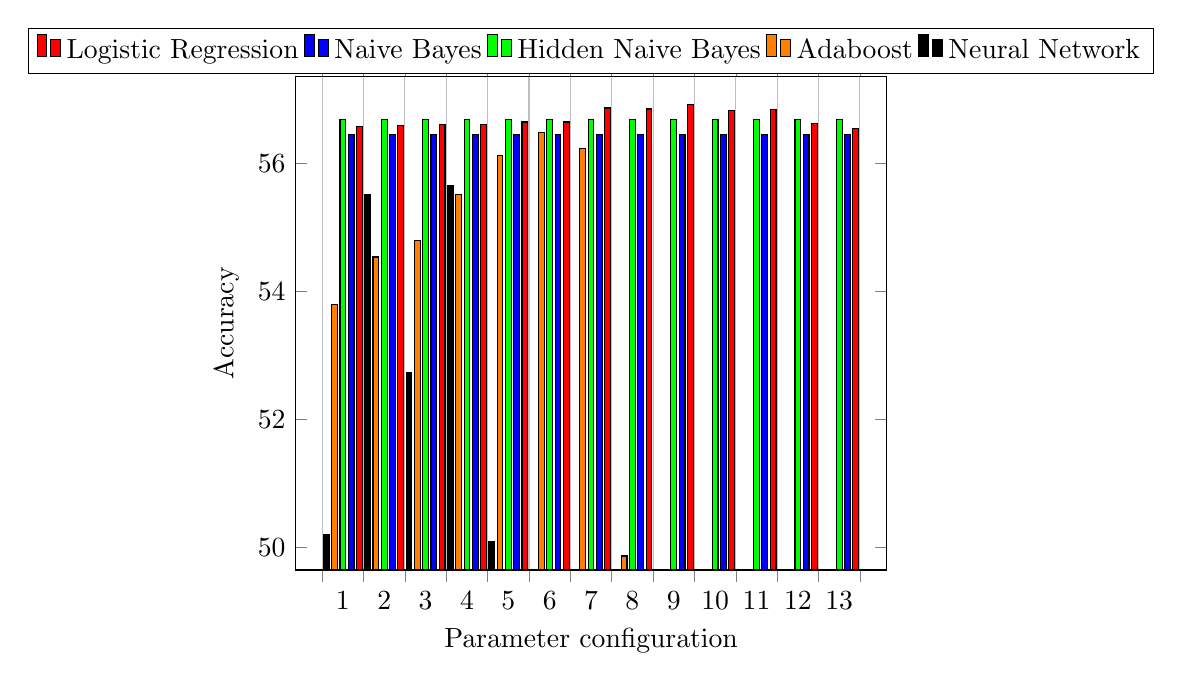
\begin{tikzpicture}
    \begin{axis}[
      x tick label style={/pgf/number format/1000 sep=},
      ylabel=Accuracy,
      xlabel=Parameter configuration,
      enlargelimits=0.05,
      legend style={at={(0.5,1.1)},
        anchor=north,legend columns=-1},
      ybar interval=0.7,
      width=.75\textwidth,
      ymin=50, ymax=57,
      ]
      \addplot[fill=red] coordinates {(13,56.5462) 
        (12,56.6218) 
        (11,56.8403) 
        (10,56.8319) 
        (9,56.916) 
        (8,56.8487) 
        (7,56.8655) 
        (6,56.6471) 
        (5,56.6471) 
        (4,56.605) 
        (3,56.605) 
        (2,56.5882) 
        (1,56.5798) 
        (0,2)
      };
      \addplot[fill=blue] coordinates {(13,56.4454) 
        (12,56.4454) 
        (11,56.4454) 
        (10,56.4454) 
        (9,56.4454) 
        (8,56.4454) 
        (7,56.4454) 
        (6,56.4454) 
        (5,56.4454) 
        (4,56.4454) 
        (3,56.4454) 
        (2,56.4454) 
        (1,56.4454) 
        (0,56.4454)
      };
      \addplot[fill=green] coordinates {(13,56.6807) 
        (12,56.6807) 
        (11,56.6807) 
        (10,56.6807) 
        (9,56.6807) 
        (8,56.6807) 
        (7,56.6807) 
        (6,56.6807) 
        (5,56.6807) 
        (4,56.6807) 
        (3,56.6807) 
        (2,56.6807) 
        (1,56.6807) 
        (0,56.6807)
      };
      \addplot[fill=orange] coordinates {(13,0) 
        (12,0) 
        (11,0) 
        (10,0) 
        (9,0) 
        (8,49.87) 
        (7,56.2269) 
        (6,56.479) 
        (5,56.1261) 
        (4,55.5126) 
        (3,54.7899) 
        (2,54.5378) 
        (1,53.7983) 
        (0,2)
      };
      \addplot[fill=black] coordinates {(13,0) 
        (12,0) 
        (11,0) 
        (10,0) 
        (9,0) 
        (8,0) 
        (7,0) 
        (6,0) 
        (5,50.1) 
        (4,55.6555) 
        (3,52.7311) 
        (2,55.5126) 
        (1,50.2101) 
        (0,0)
      };
      \legend{Logistic Regression,Naive Bayes,Hidden Naive Bayes,Adaboost,Neural Network}
    \end{axis}
  \end{tikzpicture}
  \caption{Test of best machine learning technique}\label{fig:besttech}
\end{figure}

\subsection{Implementation comparison}
To test if Apache Sparks PySpark implementation of logistic regression is implemented properly, it is compared to the equivalent implementations in Weka and R. The data consists of 5000 matches where Weka uses a sparse presentation, while R uses a dense and PySpark the raw file with JSON elements. As seen in \Cref{tab:impl_results}, the implementations are close to equal, the minor differences could be caused by differences in the parameter settings. However these results confirm that all implementations are acceptable and further testing can be performed in any of the environments.

\begin{table}[!htb]
  \centering
  \begin{tabular}{|l|c|}
    \hline
    Implementation  & Accuracy  \\
    \hline
    Weka & 55\%  \\
    R & 55\%\\
    PySpark & 53\%\\ 
    \hline
  \end{tabular}
  \caption{Implementation comparison results}
  \label{tab:impl_results}
\end{table}

\subsection{Feature representation test}
Features can be presented in many different ways and this test is constructed to finding the best way to that. The representations that will be tested are the methods presented in \Cref{sec:representationoffeatures}. The test was done on an increasing number of matches with all the different methods to check how they hold up with much data. As the result, shown in \Cref{fig:feat-rep}, indicates, method 1 and 4 are very close, but method 1 being slightly above method 4 majority of the time, which is the reason for us choosing method 1.

\begin{figure}[!htb]
  \centering
  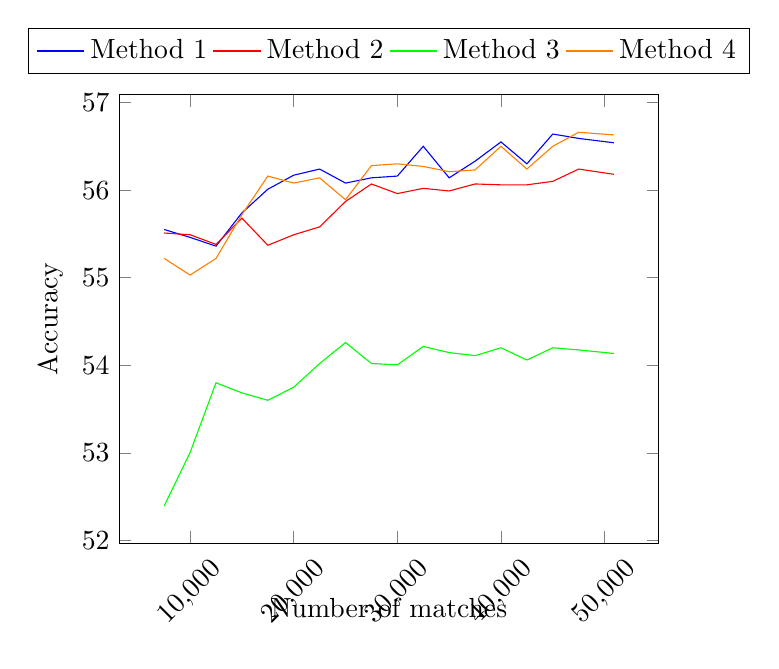
\begin{tikzpicture}[] 
    \begin{axis}[
      xlabel=Number of matches, 
      ylabel=Accuracy,
      xtick={10000,20000,30000,40000,50000},
      xticklabel style={rotate=45,anchor=near xticklabel},
      scaled x ticks=false,
      x label style={at={(axis description cs:0.5,-0.1)},anchor=north},
      legend style={at={(0.5,1.15)},
        anchor=north,legend columns=-1},] 
      \addplot[color=blue] coordinates { 
        (7500, 55.55)
        (10000, 55.46)
        (12500, 55.36)
        (15000, 55.74)
        (17500, 56.01)
        (20000, 56.17)
        (22500, 56.24)
        (25000, 56.08)
        (27500, 56.14)
        (30000, 56.16)
        (32500, 56.50)
        (35000, 56.14)
        (37500, 56.33)
        (40000, 56.55)
        (42500, 56.30)
        (45000, 56.64)
        (47500, 56.59)
        (50901, 56.54)
      };
      \addplot[color=red] coordinates { 
        (7500, 55.51)  
        (10000, 55.49)
        (12500, 55.38)
        (15000, 55.68)
        (17500, 55.37)
        (20000, 55.49)
        (22500, 55.58)
        (25000, 55.87)
        (27500, 56.07)
        (30000, 55.96)
        (32500, 56.02)
        (35000, 55.99)
        (37500, 56.07)
        (40000, 56.06)
        (42500, 56.06)
        (45000, 56.10)
        (47500, 56.24)
        (50901, 56.18)
      };
      \addplot[color=green] coordinates { 
        (7500, 52.395)  
        (10000, 53.005)
        (12500, 53.80)
        (15000, 53.685)
        (17500, 53.60)
        (20000, 53.75)
        (22500, 54.02)
        (25000, 54.26)
        (27500, 54.02)
        (30000, 54.005)
        (32500, 54.215)
        (35000, 54.145)
        (37500, 54.11)
        (40000, 54.20)
        (42500, 54.06)
        (45000, 54.20)
        (47500, 54.175)
        (50901, 54.135)
      };
      \addplot[color=orange] coordinates {
        (7500, 55.22)  
        (10000, 55.03)
        (12500, 55.22)
        (15000, 55.72)
        (17500, 56.16)
        (20000, 56.08)
        (22500, 56.14)
        (25000, 55.89)
        (27500, 56.28)
        (30000, 56.30)
        (32500, 56.27)
        (35000, 56.21)
        (37500, 56.23)        
        (40000, 56.50)
        (42500, 56.24)
        (45000, 56.50)
        (47500, 56.66)
        (50901, 56.63)
      };
      \legend{Method 1, Method 2, Method 3, Method 4}
    \end{axis} 
  \end{tikzpicture}
  \caption{Test for representation of features}\label{fig:feat-rep}
\end{figure}

\subsection{Feature tests}
Some features might be more expressive than others, and finding the set of features that will yield the best result is imperative.


\subsection{Big data improvements}
To test if big data gives an improvement when predicting the outcome of a match, the same features and method where used on an increasing sized data starting from 1000 matches. After the model was made, it was tested on the training data, as a $\frac{2}{3}$-split and finally cross-validation. And as seen on \Cref{fig:bigdata} ... %Udfyld når vi har flere tal fra clusteren. //Funder

\begin{figure}[!htb]
  \centering
  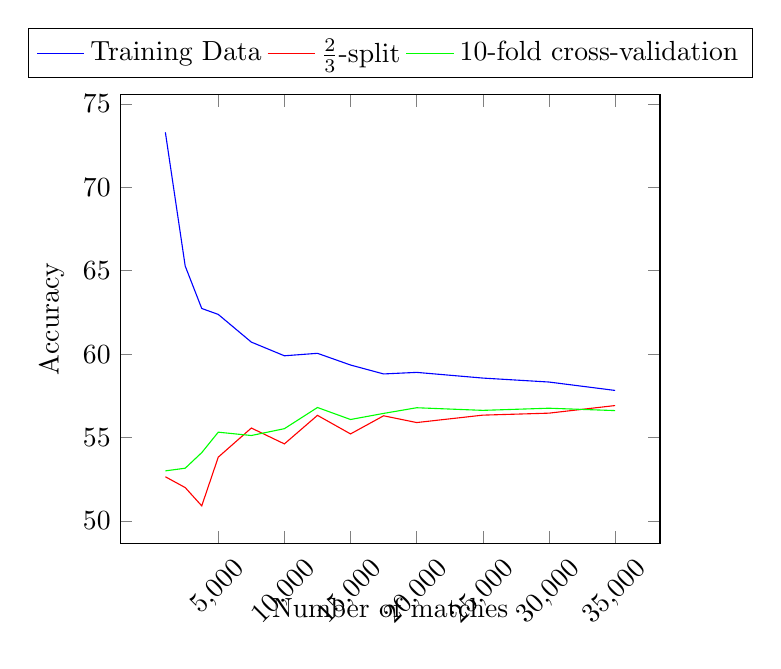
\begin{tikzpicture}[] 
    \begin{axis}[
      xlabel=Number of matches, 
      ylabel=Accuracy,
      xtick={5000,10000,15000,20000,25000,30000,35000},
      xticklabel style={rotate=45,anchor=near xticklabel},
      scaled x ticks=false,
      x label style={at={(axis description cs:0.5,-0.1)},anchor=north},
      legend style={at={(0.5,1.15)},
        anchor=north,legend columns=-1},] 
      \addplot[color=blue] coordinates {
        (1000, 73.3)   	
        (2500,65.28)  	
        (3750,62.7367)	
        (5000,62.38)
        (7500,60.72)
        (10000,59.9)
        (12500,60.048)
        (15000,59.3467)
        (17500,58.8114)
        (20000,58.905)
        (25000,58.564)
        (30000,58.3267)
        (35000,57.8229)
      };
      \addplot[color=red] coordinates {
        (1000,52.6471)
        (2500,52)
        (3750,50.902)
        (5000,53.8235)
        (7500,55.5686)
        (10000,54.6176)
        (12500,56.3294)
        (15000,55.2157)
        (17500,56.3025)
        (20000,55.8971)
        (25000,56.3412)
        (30000,56.4608)
        (35000,56.916)
      };
      \addplot[color=green] coordinates {
        (1000,53)
        (2500,53.16)
        (3750,54.0944)
        (5000,55.32)
        (7500,55.12)
        (10000,55.53)
        (12500,56.8)
        (15000,56.08)
        (17500,56.4457)
        (20000,56.785)
        (25000,56.628)
        (30000,56.7567)
        (35000,56.6143)
      };
      \legend{Training Data, $\frac{2}{3}$-split, 10-fold cross-validation}
    \end{axis} 
  \end{tikzpicture}
  \caption{Test for representation of features}\label{fig:bigdata}
\end{figure}

\subsection{Speed up}
This test is constructed to show that an increasing number of nodes increases the computation speed. As seen in \Cref{sec:clustersetup}, the cluster consists of 4 nodes, this means the test will be run with the master and either 1, 2 or 3 nodes. The data for this test be the same to make the results comparable.

\begin{table}[!htb]
  \centering
  \begin{tabular}{|c|c|}
    \hline
    Number of nodes & Time taken\\
    \hline
    1 & 42.1 \\
    2 & 42.2 \\
    3 & 42.3 \\
    \hline
  \end{tabular}
  \caption{Speed up test results}\label{tab:speedup}
\end{table}

%%% Local Variables:
%%% mode: latex
%%% TeX-master: "../main"
%%% End:
